

\documentclass{tex/sig-alternate-2013}

\usepackage[T1]{fontenc}
\usepackage{comment}
\usepackage{adjustbox}
\usepackage[usenames,dvipsnames]{color}
\usepackage{color}
\usepackage{textcomp}
\usepackage{mathabx}
%\usepackage{enumerate}
\usepackage{hyperref} 
\usepackage{array} 
\usepackage{graphicx} 
\usepackage{booktabs} 
\usepackage{pifont} 
\usepackage{rotating} 
\usepackage{color} 
\usepackage{tabularx} 
\usepackage{amssymb}
\usepackage{enumitem}
 
\newcommand*\rot{\rotatebox{90}} 

\newcommand{\todo}[1]{{\color{red}{#1}}}
\newfont{\mycrnotice}{ptmr8t at 7pt}
\newfont{\myconfname}{ptmri8t at 7pt}
\let\crnotice\mycrnotice%
\let\confname\myconfname%

\permission{Permission to make digital or hard copies of all or part of this work for personal or classroom use is granted without fee provided that copies are not made or distributed for profit or commercial advantage and that copies bear this notice and the full citation on the first page. Copyrights for components of this work owned by others than ACM must be honored. Abstracting with credit is permitted. To copy otherwise, or republish, to post on servers or to redistribute to lists, requires prior specific permission and/or a fee. Request permissions from permissions@acm.org.}
\conferenceinfo{BigSystem 2014,}{June 23, 2014, Vancouver, BC, Canada.}
\copyrightetc{Copyright 2014 ACM \the\acmcopyr}
\crdata{978-1-4503-2909-5/14/06\ ...\$15.00.\\
http://dx.doi.org/10.1145/2609441.2609638}

\clubpenalty=10000 
\widowpenalty = 10000

\begin{document}

\title{Accessing Multiple  Clouds with Cloudmesh} 
\numberofauthors{5} 
\author{
% 1st. author
\alignauthor
Gregor von Laszewski\titlenote{Corresponding author.}\\
       \affaddr{School of Informatics and Computing, Indiana University}\\
       \affaddr{919 E. 10th Street}\\
       \affaddr{Bloomington IN 47408, U.S.A.}\\ 
       \email{laszewski@gmail.com} 
% 2nd. author
\alignauthor
Fugang Wang \\
       \affaddr{School of Informatics and Computing, Indiana University}\\
       \affaddr{919 E. 10th Street}\\
       \affaddr{Bloomington IN 47408, U.S.A.}\\ 
% 3rd. author
\alignauthor Hyungro Lee\\
       \affaddr{School of Informatics and Computing, Indiana University}\\
       \affaddr{919 E. 10th Street}\\
       \affaddr{Bloomington IN 47408, U.S.A.}\\ 
\and  % use '\and' if you need 'another row' of author names
% 4th. author
\alignauthor Heng Chen\\
       \affaddr{School of Informatics and Computing, Indiana University}\\
       \affaddr{919 E. 10th Street}\\
       \affaddr{Bloomington IN 47408, U.S.A.}\\ 
% 5th. author
\alignauthor Geoffrey C. Fox\\
       \affaddr{School of Informatics and Computing, Indiana University}\\
       \affaddr{919 E. 10th Street}\\
       \affaddr{Bloomington IN 47408, U.S.A.}\\ 
}

\date{27 April 2014}

\maketitle
\begin{abstract}
\todo{READ}

We present the design of a toolkit that can be used by users and administrators to manage virtual machines on multi-cloud environments.  It can be run by individual users or offered as a service to a shared user community. We have practically, demonstrated its use as part of a FutureGrid service allowing users of FutureGrid to utilize such a service. Furthermore, we are discussing implications and solutions for a unified metrics system assisting the users to find and utilize resources appropriate for their applications. Lastly we discuss how to move such a multi-cloud environment forward by integrating clouds managed by the community or are offered as public clouds. This includes the introduction of a mutual trust agreements on user and project basis. We have developed a number of components that support the creation of such a multi-cloud environment. This system is known as Cloudmesh and has been used in practice to achieve virtual machine management in multiple clouds. An important distinguishing factor of Cloudmesh is that it also allows the use of bare metal provisioning for supporting service providers and authorized users, offering services beyond those available by typical clouds.

\end{abstract}

% A category with the (minimum) three required fields
\category{C.2.4}{Distributed Systems}{Cloud Computing}

\terms{Computer-Communication Networks}

\keywords{Cloud, multi-cloud, federated clouds, FutureGrid, cloudmesh}

\section{Introduction}

\todo{READ} 

Cloud computing has become an important factor for managing infrastructure by research organizations and industry. Users and organizations are faced with a variety of solutions that may support their needs. Such offerings include a variety of Infrastructure as a Service (IaaS) frameworks. The choice between them provides a significant risk of investment and needs to be conducted carefully. The community has the choice to either use public clouds or set up their own private clouds. Public clouds are offered by large providers such as Amazon, Microsoft, Google, Rackspace, HP, and others. Private clouds are set up by the internal Information Technology (IT) departments and made available as part of the general IT infrastructure. Two aspects result from this availability that need to be considered. First, which of the many Infrastructures should be chosen? Second, can the multitude of IaaS service offerings be leveraged and instead of choosing one a service can be offered that utilizes multiple of them. Furthermore, we have to consider that the IaaS frameworks to deploy private clouds are evolving and that extensions may be needed that are not yet offered by the frameworks to adequately address the requirements posed by advanced IT service infrastructures of research organizations.

In this paper we will present the design and implementation of a toolkit that addresses some of the points raised here.  The paper is structured as follows. First we discuss the important terminology used in this paper (Section \ref{S:terminology}).  Next we analyze the requirements in more detail (Section \ref{S:requirements}) and summarize some related work (Section \ref{S:related}).  The requirements motivate our design (Section \ref{S:design}) and implementation (Section \ref{S:implementation}).  We focus on two aspect of the cloudmesh features, namely dynamic provisioning/ rain, as well as Lastly we present our conclusion (Section \ref{S:conclusion})

\subsection{Terminology} \label{S:terminology}

\todo{READ}
We will be using the following definitions throughout the paper:

\begin{description}[leftmargin=*,itemsep=0pt,topsep=0pt]

\item[Public cloud:]  a service provider makes resources available to users over the public Internet. This includes compute, storage, and applications. FutureGrid offers to its users a public cloud. 

\item[Private cloud:] access to services may be having additional restrictions. Restrictions could include a limited set of authorized users to the services offered or  possible restrictions of exposing services on the public internet. FutureGrid offers the ability to set up private clouds for special projects. Examples include modified OpenStack deployments or reserved resources for classes.

\item[Hybrid cloud:] a combination of public and private clouds. 

\item[Multi-cloud:] access to a number of different clouds that may even use different IaaS or PaaS offerings. 

\item[HPC service:] a cloud service that allows the ability to run high performance computing jobs, for example on a compute cluster offering MPI. 

\item[Provisioning:] a set of instructions to install the operating system, data and software to enable access to it. 

\item[Rain:] an advanced set of instructions that not only provisions the operating system, but allows the deployment and configuration of useful and complex services to be run on one or multiple machines in order to provide a service utilizing potentially distributed resources or services.  It also contains the ability to re-provision servers and services, that is services may be suspended and the resources used to run the service may be used by other services.

\item[Provider consortium:] is a (virtual) organization that integrates resources from multiple providers. We also can refer to such a consortium as a multi-cloud Grid.

\end{description}



%%%%%%%%%%%%%%%%%%%%%%%%%%%%%%%%%%%%%%%%%%%%%%%%%%%%%%%%%%%%%%%%%%%%%%
\section{Requirements} \label{S:requirements}).
%%%%%%%%%%%%%%%%%%%%%%%%%%%%%%%%%%%%%%%%%%%%%%%%%%%%%%%%%%%%%%%%%%%%%%


TBD


%%%%%%%%%%%%%%%%%%%%%%%%%%%%%%%%%%%%%%%%%%%%%%%%%%%%%%%%%%%%%%%%%%%%%%
\section{Related Work}\label{S:related}
%%%%%%%%%%%%%%%%%%%%%%%%%%%%%%%%%%%%%%%%%%%%%%%%%%%%%%%%%%%%%%%%%%%%%%

\todo{READ}

It is not possible to provide an extensive overview of related research due to space limitations of this paper. Instead we provide examples of activities that address similar but not the same issues as our work.

\begin{description}[leftmargin=0pt,itemsep=0pt,topsep=0pt]

\item[Phantom] \cite{phantom12,www-phantom} is a tools that monitors the health of resources and automatically provisions and configures new ones based on demand. IT is designed to automatically (a) provisioning new resources to counteract failures or (b) react to increasing demand reducing constant attention and repetitive task that can be automated.  

  Our effort is different as our framework is targeted not only on the user initiated federation of resources, the access to the native protocols that are not exposed in libcloud as used by this effort and relying on the EC2 protocol, as well as the concept of access to bare metal provisioning. Furthermore, our framework includes the ability to provide a holistic cloud usage service that can be used to develop holistic scheduling algorithms for better utilization.

\item[RightScale] \cite{Rightscale} enables users to manage multi-cloud infrastructure by migrating workloads between private clouds and public clouds. RightScale interfaces with a wide variety of clouds including Amazon Web Services (AWS), Rackspace Cloud, Windows Azure, and Google Compute Engine. In addition it also offers a cloud cost estimator allowing customers to assess expenses they are charged by comparing their workload on various cloud providers.

Our effort is different as it is an open source toolkit and allows the deployment not only as a hosted service managed by one entity, but allows the deployment by a provider, provider consortium, or even the user. 

%\item[StarCluster] \cite{www-starcluster} StarCluster is a toolkit to
%  simplify the process of building, configuring, and managing clusters
%  of virtual machines on Amazon's EC2 cloud. 

\end{description}

Other research efforts include theoretical definitions for Cloud Federation \cite{kurze2011cloudfederation} or are relying on a single IaaS such as the efforts planed for future versions of OpenStack. Standard efforts such as OCCI provide naturally an interesting approach of multi-cloud interoperability, but at the same time may hinder the innovation brought forward by individual IaaS offerings. We see such difference for example in the difference between the OpenStack and EC2 API's leading for example to limitations in the functionality of Phantom while relying on the EC2 quasi-standard protocol.

\todo{DO NOT READ TILL YOU FIND ANOTHER READ}

\subsection{FutureGrid}



FutureGrid \cite{las2010gce,las12fg-bookchapter} ``is a project led by Indiana University and funded by the National Science Foundation (NSF) to develop a high performance grid test bed that will allow scientists to collaboratively develop and test innovative approaches to parallel, grid, and cloud computing. FutureGrid will provide the infrastructure to researchers that allows them to perform their own computational experiments using distributed systems. The goal is to make it easier for scientists to conduct such experiments in a transparent manner.  FutureGrid users will be able to deploy their own hardware and software configurations on a public/private cloud, and run their experiments. They will be able to save their configurations and execute their experiments using the provided tools. The FutureGrid test bed is composed of a high speed network connecting distributed clusters of high performance computers. FutureGrid employs virtualization technology that will allow the test bed to support a wide range of operating systems.''



FutureGrid contains a number compute resources organized as part of clusters with different types and size. They are interconnected with up to a 10GB Ethernet among its sites. The sites include Indiana University, University of Chicago, San Diego Supercomputing Center, Texas Advanced Computing Center, and University of Florida.  In total 481 compute servers with 1126 CPUs and 4496 Cores are offered. In addition it offers also 448 GPU cores. The total RAM is about 21.5TB. Secondary storage is about 1PB. A more detailed description of the resources is provided in \cite{vonLaszewski-bigdata-bookchapter2014}

FutureGrid offers a very rich environment to its users. We distinguish the following categories: Cloud PaaS, IaaS, GridaaS, HPCaaS, TestbedaaS.

FutureGrid provides an advanced framework to manage user and project affiliation and propagates this information to a variety of subsystems constituting the FG service infrastructure. This includes operational services to deal with authentication, authorization and accounting. In particular we have developed a unique metric framework that allows us to create usage reports from our entire Infrastructure as a Service frameworks. Repeatable experiments can be created with a number of tools including Pegasus, Precip and Cloudmesh. Provisioning of services and images can be conducted by RAIN \cite{imagemanagement,fg-1295}. Infrastructure monitoring is enabled via Nagios \cite{nagios}, Ganglia \cite{ganglia}, and Inca \cite{inca} and our own cloud metric system \cite{las08federated-cloud}.
Within the traditional high performance computing services FG offers a traditional MPI/batch queuing system and a virtual large memory system that are beneficial for big data calculations.


One of the main features of FutureGrid is to offer its users a variety of infrastructure as a service frameworks \cite{comparisoncloud,las2011virt} including OpenStack, Eucalyptus, and Nimbus. These frameworks provide Based on our experience with FutureGrid over the last couple of years, it is advantageous to offer a mixed operation model. This includes a standard production cloud that operates on-demand, but also a set of cloud instances that can be reserved for a particular project. We have conducted this for several projects in FutureGrid, including those that required dedicated access to resources as part of big data research such as classes \cite{fg405,fg368} or research projects with extremely large virtual machines \cite{fg298}.

\subsection{Federation}

Cloud federation

Account based federation

Administrative federation

\url{http://www.egi.eu/infrastructure/cloud/}


\cite{kurze2011cloudfederation}




%%%%%%%%%%%%%%%%%%%%%%%%%%%%%%%%%%%%%%%%%%%%%%%%%%%%%%%%%%%%%%%%%%%%%%
\section{Design}\label{S:design}
%%%%%%%%%%%%%%%%%%%%%%%%%%%%%%%%%%%%%%%%%%%%%%%%%%%%%%%%%%%%%%%%%%%%%%

TBD

%%%%%%%%%%%%%%%%%%%%%%%%%%%%%%%%%%%%%%%%%%%%%%%%%%%%%%%%%%%%%%%%%%%%%%
\section{Implementation}\label{S:implementation}
%%%%%%%%%%%%%%%%%%%%%%%%%%%%%%%%%%%%%%%%%%%%%%%%%%%%%%%%%%%%%%%%%%%%%%

TBD

%%%%%%%%%%%%%%%%%%%%%%%%%%%%%%%%%%%%%%%%%%%%%%%%%%%%%%%%%%%%%%%%%%%%%%
\section{Status and Future Work}
%%%%%%%%%%%%%%%%%%%%%%%%%%%%%%%%%%%%%%%%%%%%%%%%%%%%%%%%%%%%%%%%%%%%%%

TBD


\section{Code}

\begin{figure}[htb]
\begin{small}
\begin{verbatim}
class ComputeBaseType:
    flavors = {}, images = {}, servers = {}
    // Methods
    def __init__(self, label, cred=None):
    def connect(self):
    def get(self, type): type in {server, images, flavors, 
                                  users, tennant}
    def refresh(self, type=None):
    def vm_create(self, name=None,
                  flavor_name=None,
                  image_id=None,
                  security_groups=None,
                  key_name=None,
                  meta=None):
    def vm_delete(self, id):
    def rename(self, old, new, id=None):
    def usage(self, start, end, format='dict'):
    def limits(self):
    def wait(self, vm_id, vm_status, seconds=2):
    def __str__(self):
    def vms(self):
    def status(self, vm_id):
    def set_credentials(self, cred):
    def keypair_list(self):
    def keypair_add(self, keyname, keycontent):
    def keypair_remove(self, keyname):
\end{verbatim}
\end{small}
\vspace{-12pt}
\caption{Abstract interface to access different virtual machine
  management functionality}
\end{figure}

\section{Cloudmesh}\label{S:cloudmesh}


At \cite{github-cloudmesh} we find an extensive set of information about Cloudmesh that is cited within this section. 
From the experience with FutureGrid we identified the need for a more tightly integrated software infrastructure addressing the need to deliver a software-defined system encompassing virtualized and bare-metal infrastructure, networks, application, systems and platform software with a unifying goal of providing Cloud Testbeds as a Service (CTaaS). This system is termed Cloudmesh to symbolize 


\begin{enumerate}[leftmargin=*,itemsep=0pt,topsep=0pt]


\item the creation of a tightly integrated mesh of services targeting multiple IaaS frameworks 


\item the ability to federate a number of resources from academia and industry. This includes existing FutureGrid infrastructure, Amazon Web Services, Azure, HP Cloud, Karlsruhe using not only one IaaS framework but various. 


\item the creation of an environment in which it becomes more easy to experiment with platforms and software services while assisting to deploy them more easily.  


\end{enumerate}


In addition to virtual resources, FutureGrid exposes bare-metal provisioning to users, but also a subset of HPC monitoring infrastructure tools. Services will be available through command line, API, and Web interfaces.


\subsection{Functionality}


Due to its integrated services Cloudmesh provides the ability to be an onramp for other clouds. It also provides information services to various system level sensors to give access to sensor and utilization data. They internally can be used to optimize the system usage. The provisioning experience from FutureGrid has taught us that we need to provide the creation of new clouds, the repartitioning of resources between services (cloud shifting), and the integration of external cloud resources in case of over provisioning (cloud bursting). As we deal with many IaaS we need an abstraction layer on top of the IaaS framework. Experiment management is conducted with workflows controlled in shells \cite{cmd3}, Python/iPython, as well as systems such as OpenStack?s Heat, Accounting is supported through additional services such as user management and charge rate management. Not all features are yet implemented. Figure \label{F:cm-func} shows the main functionality that we target at this time to implement.


\begin{figure}[htb]
  \centering
    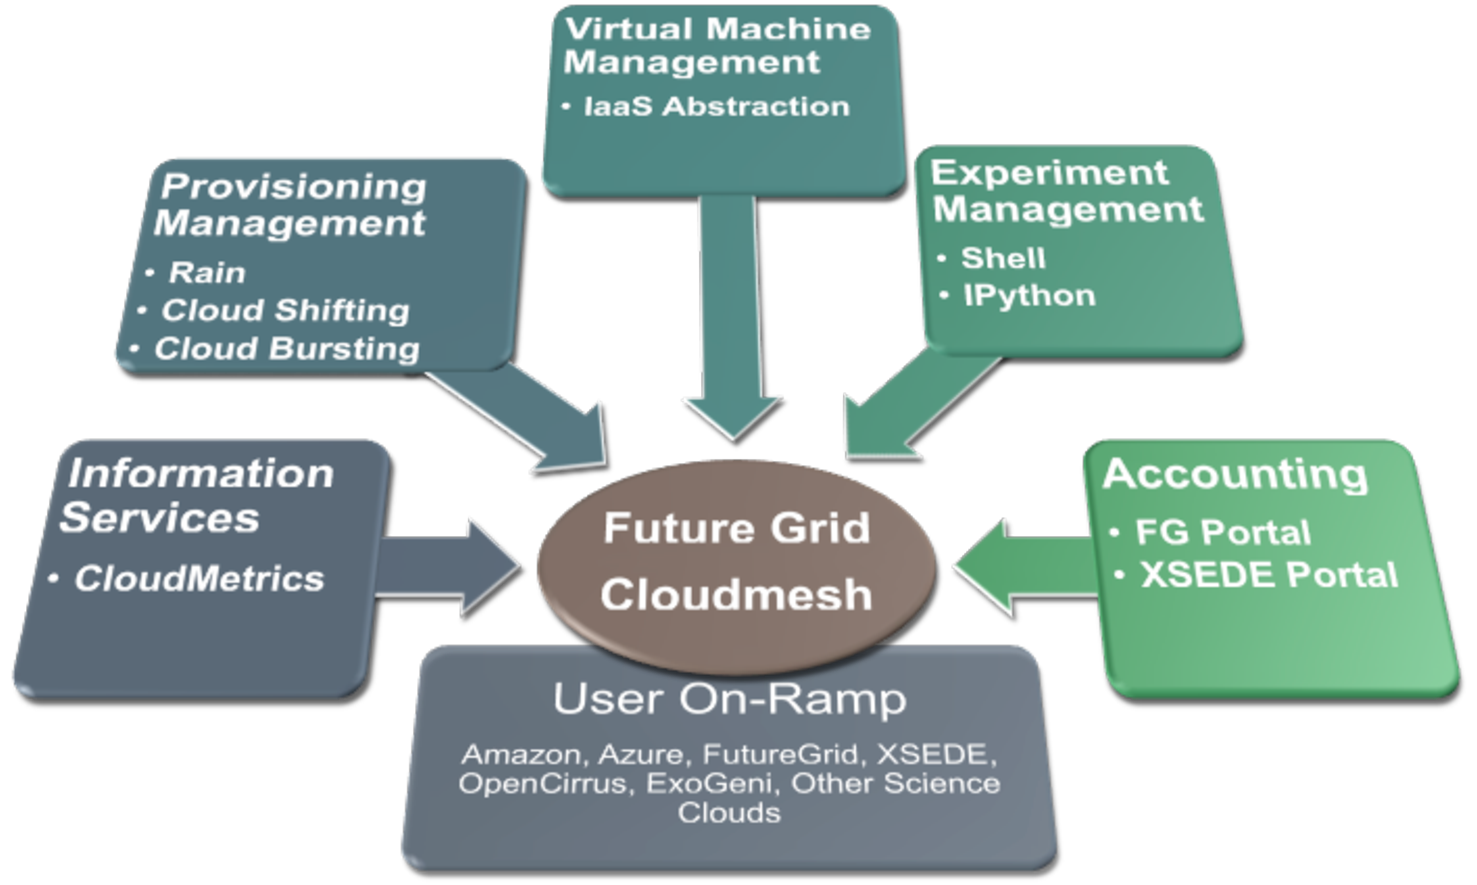
\includegraphics[width=1.0\columnwidth]{images/cm-functionality.pdf}
  \caption{CM Functionality.}\label{F:cm-func}
\end{figure}




\subsection{Architecture}


The three layers of the Cloudmesh architecture include a Cloudmesh Management Framework for monitoring and operations, user and project management, experiment planning and deployment of services needed by an experiment, provisioning and execution environments to be deployed on resources to (or interfaced with) enable experiment management, and resources.


\begin{figure}[htb]
  \centering
    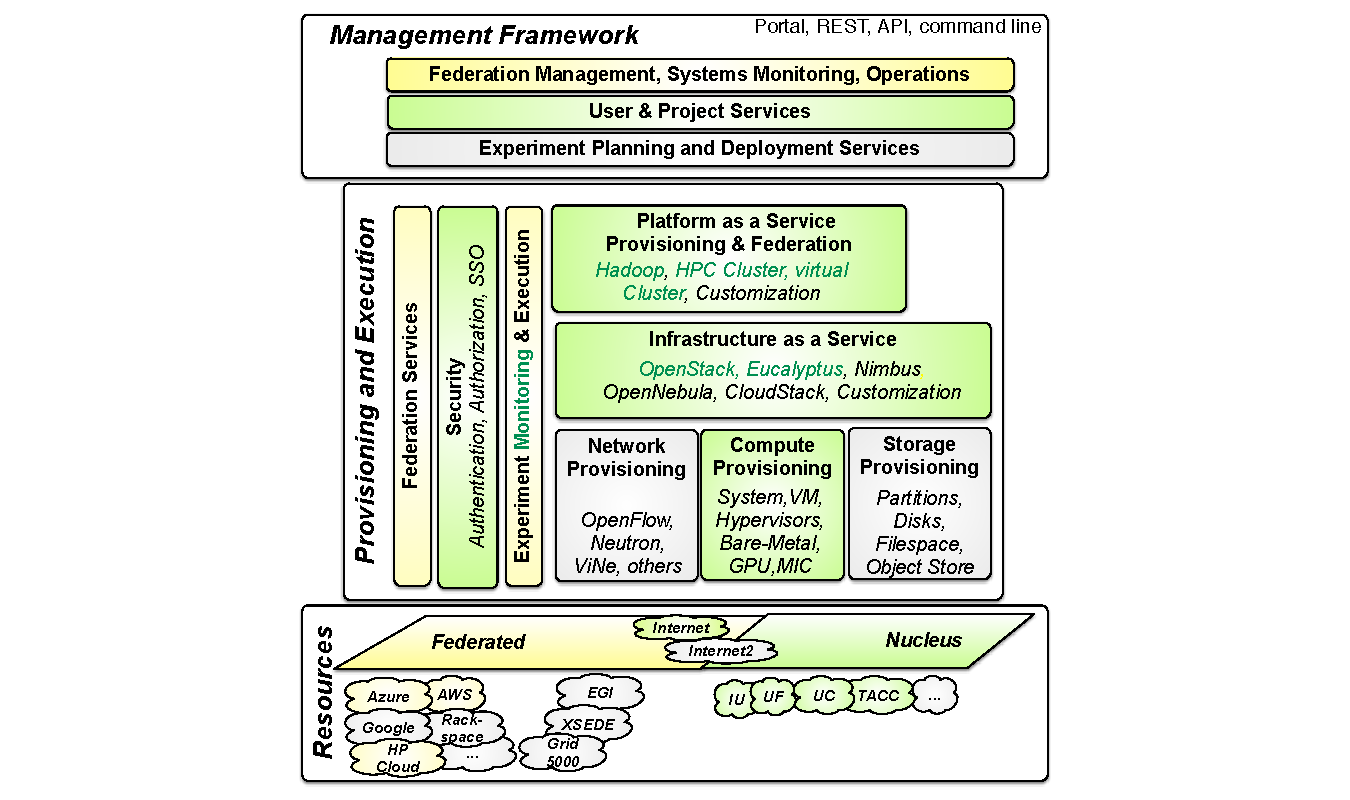
\includegraphics[width=1.0\columnwidth]{images/cm-arch.pdf}
  \caption{CM Architecture.}
\end{figure}


\paragraph{System Monitoring and Operations.}


The management framework contains services to facilitate FutureGrid day-to-day operation, including federated or selective monitoring of the infrastructure. Cloudmesh leverages FutureGrid for the operational services and allows administrators to view ongoing system status and experiments, as well as interact with users through ticket systems and messaging queues to inform subscribed users on the status of the system.
The Cloudmesh management framework offers services that simplify integration of resources in the FutureGrid nucleus or through federation. This includes, for user management, access to predefined setup templates for services in enabling resource and service provisioning as well as experiment execution. To integrate IaaS frameworks Cloudmesh offers two distinct services:


(a) a federated IaaS frameworks hosted on FutureGrid,
(b) the availability of a service that is hosted on FutureGrid, allowing the integration of IaaS frameworks through user credentials either registered by the users or automatically obtained from our distributed user directory.


For (b) several toolkits exist to create user-based federations, including our own abstraction level which supports interoperability via libcloud, but more importantly it supports directly the native OpenStack protocol and overcomes limitations of the EC2 protocol and the libcloud compatibility layer. Plugins that we currently develop will enable access to clouds via firewall penetration, abstraction layers for clouds with few public IP addresses and integration with new services such as OpenStack Heat. We successfully federated resources from Azure, AWS, the HP cloud, Karlsruhe Institute of Technology Cloud, and four FutureGrid clouds using various versions of OpenStack and Eucalyptus. The same will be done for OpenCirrus resources at GT and CMU through firewalls or proxy servers.
Additional management flexibility will be introduced through automatic cloud-bursting and shifting services. While cloud bursting will locate empty resources in other clouds, cloud shifting will identify unused services and resources, shut them down and provision them with services that are requested by the users. We have demonstrated this concept in 2012 moving resources for more than 100 users to services that were needed based on class schedules. A reservation system will be used to allow for reserved creation of such environments, along with improvements of automation of cloud-shifting.


\paragraph{User and Project Services}


FutureGrid user and project services simplify the application processes needed to obtain user accounts and projects. We have demonstrated in FutureGrid the ability to create accounts in a very short time, including vetting projects and users -- allowing fast turn-around times for the majority of FutureGrid projects with an initial startup allocation. Cloudmesh reuses this infrastructure and also allows users to manage proxy accounts to federate to other IaaS services to provide an easy interface to integrate them.


\paragraph{Accounting and App Store}


To lower the barrier of entry Cloudmesh will be providing a shopping cart which will allow checking out of predefined repeatable experiment templates. A cost is associated with an experiment making it possible to engage in careful planning and to save time by reusing previous experiments. Additionally, the Cloudmesh App Store may function as a clearing-house of images, image templates, services offered and provisioning templates. Users may package complex deployment descriptions in an easy parameter/form-based interface and other users may be able to replicate the specified setup with.
Due to our advanced Cloudmesh Metrics framework we are in the position to further develop an integrated accounting framework allowing a usage cost model for users and management to identify the real impact of an experiment on resources. This will be useful to avoid overprovisioning and inefficient resource usage. The cost model will be based not only on number of core hours used, but also the capabilities of the resource, the time, and special support it takes to set up the experiment. We will expand upon the metrics framework of FutureGrid that allows measuring of VM and HPC usage and associate this with cost models. Benchmarks will be used to normalize the charge models.


\paragraph{Networking}


in{ceWe have a broad vision of resource integration in FutureGridources be with systems offering different levels of control from bare metal to use of a portion of a resource. Likewise, we must utilize networks offering various levels of control, from standard IP connectivity to completely configurable SDNs as novel cloud architectures will almost certainly leverage NaaS and SDN alongside system software and middleware. FutureGrid resources will make use of SDN using OpenFlow whenever possible and the same level of networking control will not be available in every location.


\paragraph{Monitoring}


To serve the purposes of CISE researchers, Cloudmesh must be able to access empirical data about the properties and performance of the underlying infrastructure beyond what is available from commercial cloud environments. To accommodate this requirement we have developed a uniform access interface to virtual machine monitoring information available for OpenStack, Eucalyptus, and Nimbus. In the future, we will be enhancing the access to historical user information. Right now they are exposed through predefined reports that we create on a regular basis. To achieve this we will also leverage the ongoing work while using the AMPQ protocol. Furthermore, Cloudmesh will provide access to common monitoring infrastructure as provided by Ganglia, Nagios, Inca, perfSonar, PAPI and others.

\subsection{Cloud Shifting}


We have already demonstrated via the RAIN tool in Cloudmesh that it is possible to easily shift resources between services. We are currently expanding upon this idea and developing more easy to use user interfaces that assist administrators and users through role and project based authentication to move resources from one service to another (see Figure \ref{F:shift}).


\begin{figure}[htb]
  \centering
    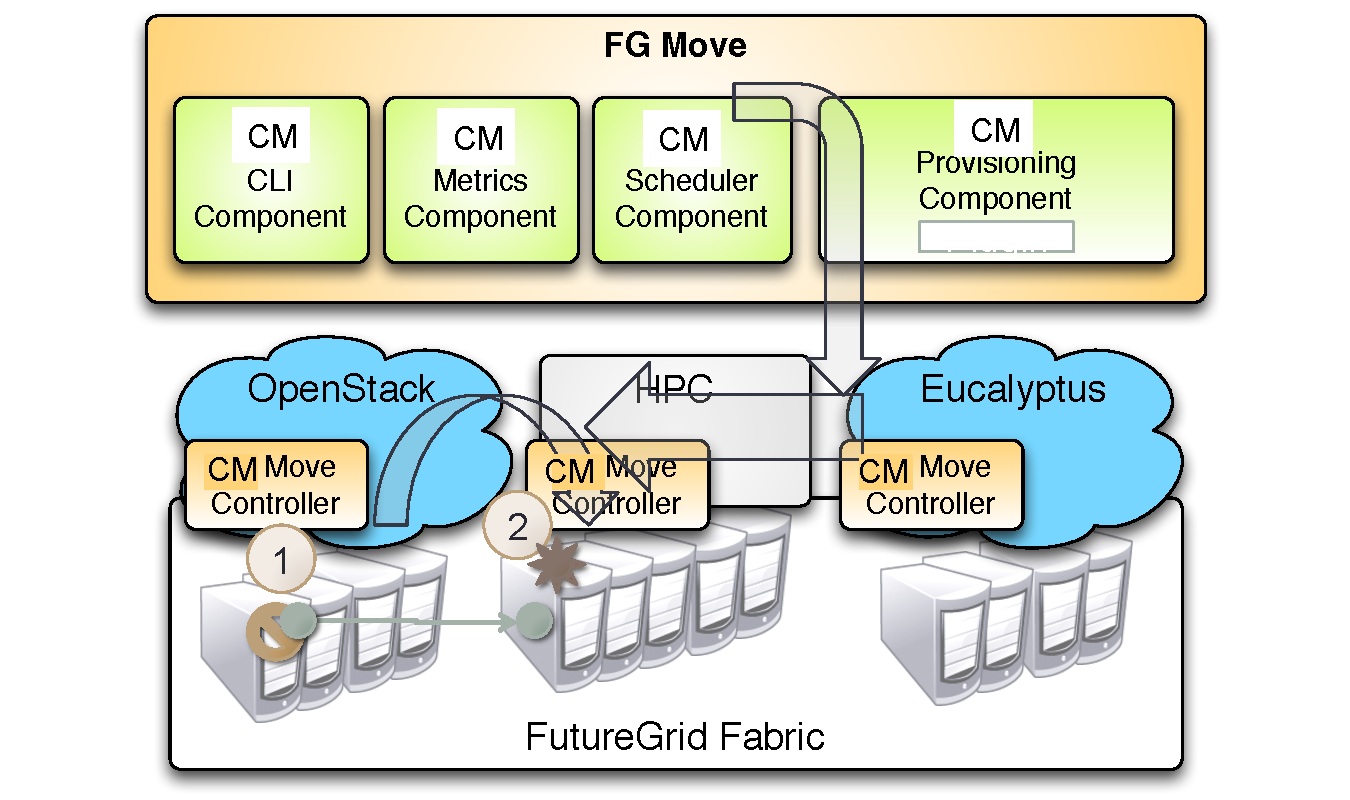
\includegraphics[width=1.0\columnwidth]{images/shift2.pdf}
  \caption{Shifting resources makes it possible to offer flexibility
    in the service distribution in case of over or underprovisioning.}\label{F:shift}
\end{figure}


\subsection{Graphical User Interface}


Despite the fact that Cloudmesh was originally a quite sophisticated command shell and command line tool, we have spend recently more time in exposing this functionality through a convenient Web interface. Some more popular views if this interface are depicted in Figure \ref{F:instances} hinting on how easy it is with a single button to create multiple VMs across a variety of IaaS. Also nice is that this not only includes resources at IU but also at external locations. Pushing this easy management in a more sophisticated experience for the user while associating one-click deployments that include the ability to deploy virtual clusters, Hadoop environments, and other more elaborate setups we provide an early prototype screenshot in Figure \ref{F:oneclick}.


\begin{figure}[htb]
  \centering
    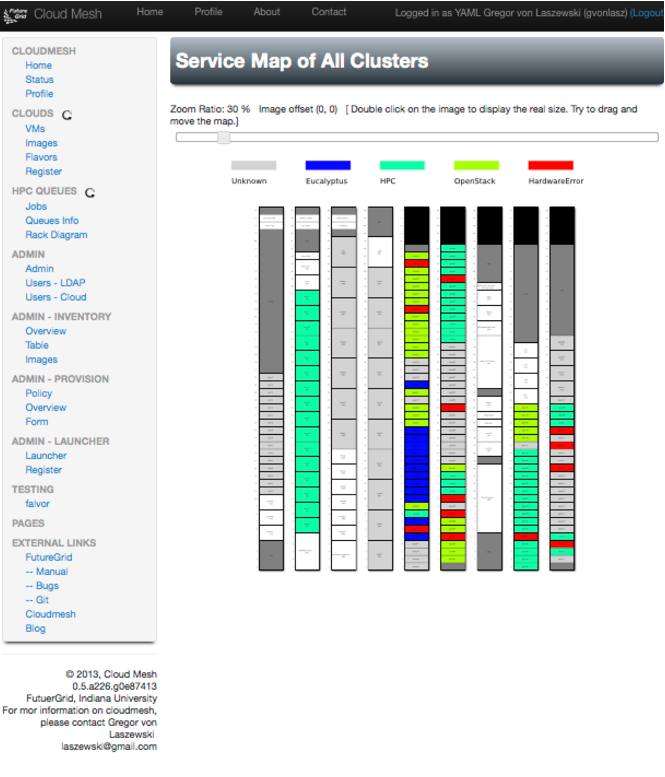
\includegraphics[width=1.0\columnwidth]{images/rainbow.pdf}
  \caption{Monitoring the Service distribution of FutureGrid with Cloudmesh.}
\end{figure}


\begin{figure}[htb]
  \centering
    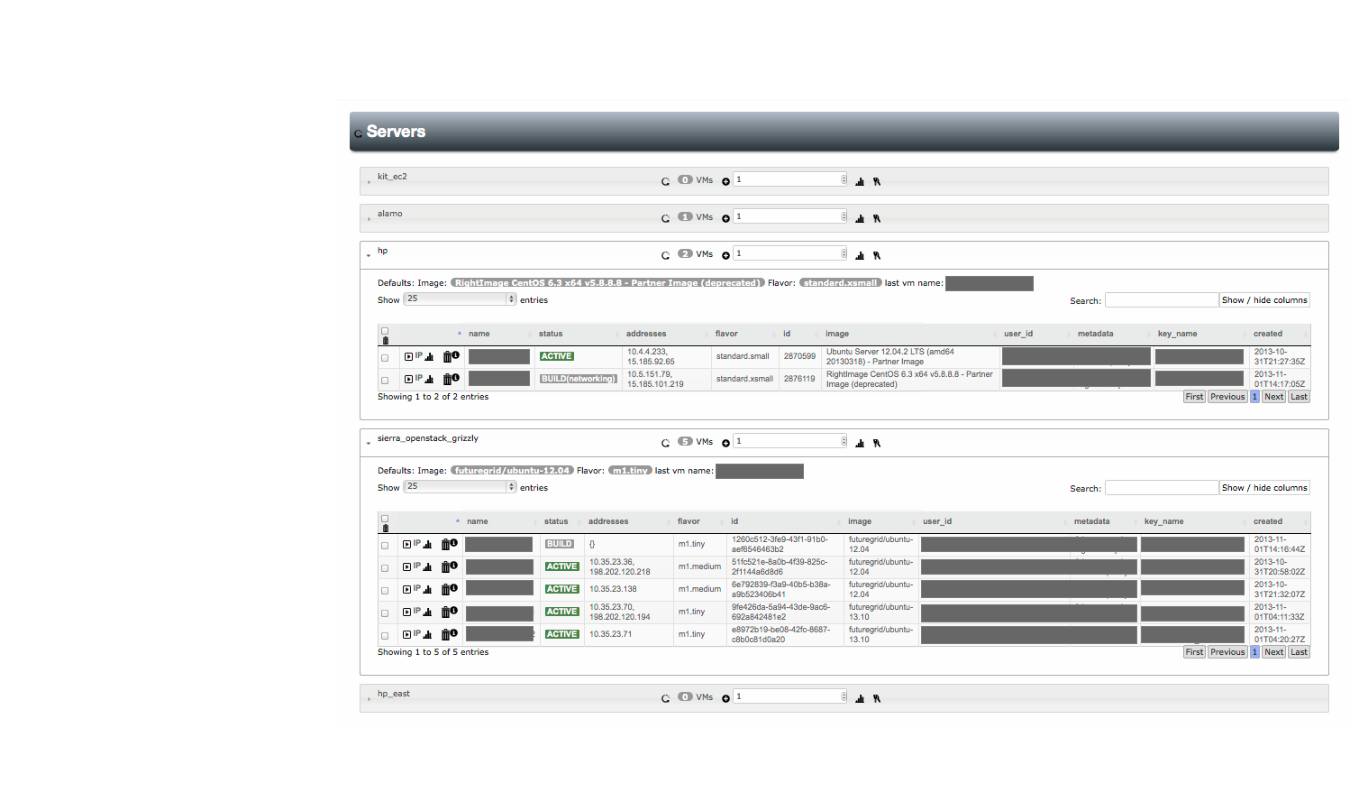
\includegraphics[width=1.0\columnwidth]{images/instances.pdf}
  \caption{Screenshot demonstrating how easy ot is to manage multible VMs accross various clouds.}\label{F:instances}
  \centering
    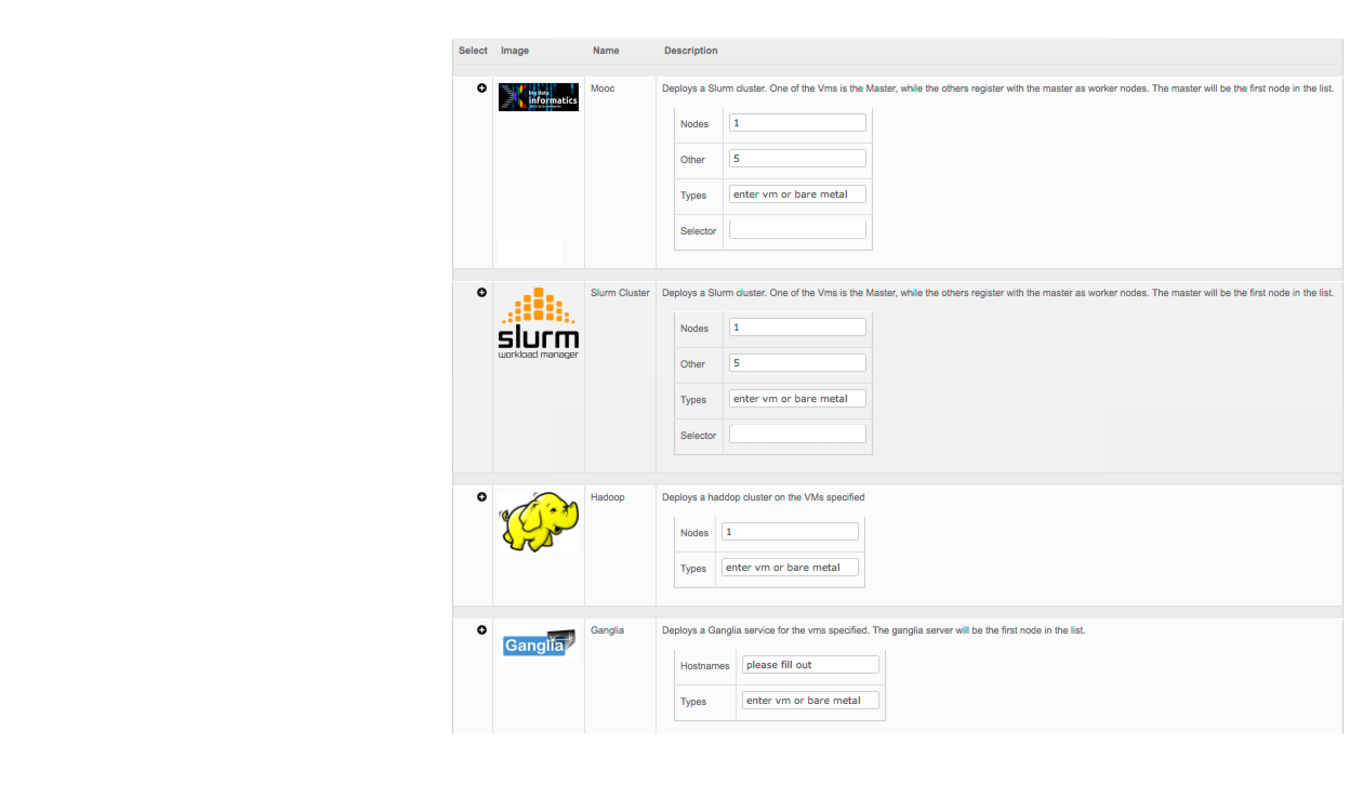
\includegraphics[width=1.0\columnwidth]{images/oneclick.pdf}
  \caption{One click deployment of platforms and sophisticated
    services that could even spawn multiple resources.}\label{F:oneclick}
\end{figure}

\subsection{Cloud Metrics}

\todo{READ}

Based on lessons learned from FutureGrid, knowledge of the resource allocation and utilization is important to provide users and administrators with a holistic view of the infrastructure in order to guide better utilization overall and on an individual basis. This is especially of interest in cloud deployments such as FutureGrid, which supports more than 380 projects and 2300 users (as of April 2014). Due to such a large user base resources could become over provisioned or are not properly utilized by the users. Among the many services that FutureGrid offers we have especially focused on IaaS including OpenStack, Eucalyptus, Nimbus, as well as batch systems to offer high performance computing capabilities.  However, for this paper we will restrict our discussion on the IaaS based monitoring components.  Other HPC related activities in regards to monitoring and metrics are discussed in \cite{ubmod,las12xdmod-kernel,las12xdmod-planing,las13xdmod,smith13info}

When FG initially started the existing IaaS frameworks such as Eucalyptus, Nimbus, and OpenStack did not provide adequate support for monitoring resource usage. Furthermore, a service with sufficient monitoring capabilities across heterogeneous cloud IaaS frameworks was not available. Hence, it was difficult to assess user utilization in a holistic fashion. Additionally, we found that some IaaS frameworks such as Nimbus, lack support for project allocations, a must have feature to support project managed allocations as is the case in almost every modern shared datacenter.  To overcome these missing features and service offerings, we developed a {\em federated cloud metric service} that aggregates the information from distributed clusters and a variety of heterogeneous IaaS services, such as OpenStack, Eucalyptus, and Nimbus. We name this service {\em Cloudmesh Metrics}.

The main components of {\em Cloudmesh Metrics} enable (a) the measurement of the resource allocation across several IaaS platforms, (b) the generation of data in regards to utilization, (c) the comparison of data via definable metrics to mine the usage statistics, (d) the display of the information through a convenient user interface, (f) the availability of a simple command line interface and shell language, and (e) the automatic creation of resource reports in printed format for arbitrary time periods.

The services offered by Cloudmesh Metrics support requirements from a variety of user communities. This includes individual users and users part of projects (Section \ref{S:user-metric}), as well as administrative users (Section \ref{S:resource-metric}).


\subsubsection{User- and Project-based Metrics Services}\label{S:user-metric} 

\todo{READ}

In order for users to use a variety of clouds it is important for them to monitor and compare their resource utilization on them. In case the usage is organized as a project the project related information needs to be exposed while being able to clearly distinguish between different projects. Furthermore we need to support an overall project view.  Thus the requirement exists to present the data to the user based on individual user utilization, group, utilization, or even experiment utilization, where a particular experiment is analyzed instead of just looking at the total utilization.

\subsubsection{Resource Provider-based Metrics Services} \label{S:resource-metric}

\todo{READ}

For the resource provider it is important to have access to a holistic view of the a variety of metrics across a the various clouds that build the multi-cloud environment as part of a provider consortium.  Summary information may be customized based on the requirements by individual users, project leads, resource providers, site managers, and funding agencies. This information is typically restricted to the actual {\em resources} for which administrative access exists in order to provide a holistic set of metrics.


\subsubsection{Metric Access for Multi-cloud Environments} 

\todo{READ}

Due to the different governance models between a private cloud managed as part of a provider consortium, and the integration of resources must be based on an access integration policy. In order to devise such a policy, we need to be aware of the hierarchical access management employed in clouds and depicted in Figure \ref{F:metric-hierarchy}.

\begin{figure}[htb]
  \centering
    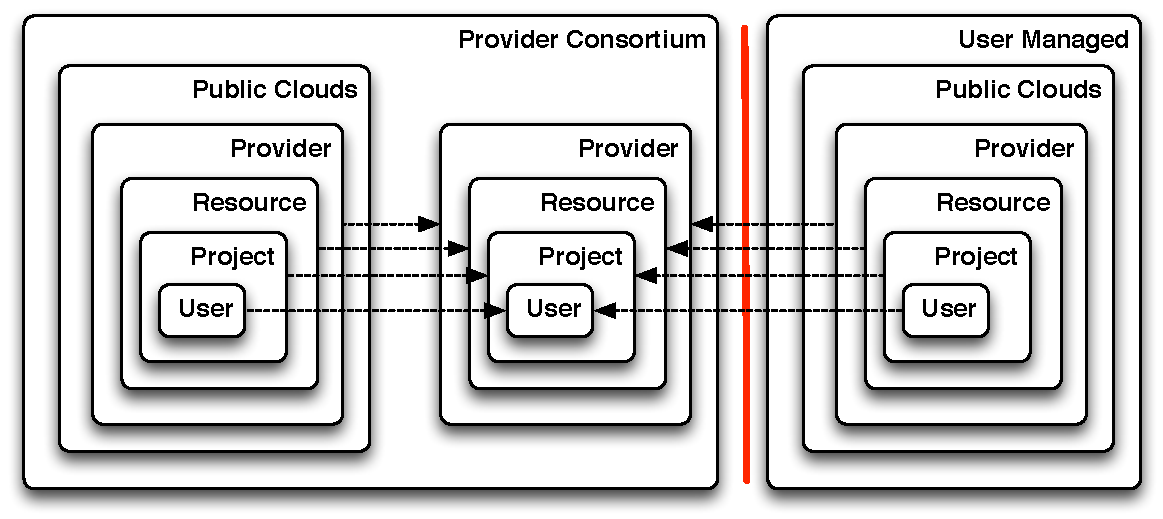
\includegraphics[width=1.0\columnwidth]{images/metric-hierarchy.pdf}
  \caption{An example of a policy to estabilsh a access public clouds as part of 
    provider and user managed multi-clouds.}
  \label{F:metric-hierarchy}
\end{figure}

\paragraph{Integration into a Provider Consortium Managed Multi-Cloud}

\newcommand{\ARROW}{$\Rightarrow$}

\todo{READ}

In the hierarchy we distinguish user \ARROW project with many users \ARROW a resource serving many projects \ARROW a Provider having many resources \ARROW and a Provider consortium with many providers.

The provider consortium has a multitude of possibilities to extend their resource offerings to its users while integrating public clouds. This could include to replicate projects on public clouds, or to assign a particular user access to an account that integrates resources in a public cloud. In case Multiple clouds are offered this integration could be replicated for them. Hence it would be possible for a Provider consortium not only to provide private clouds as part of a multi-cloud environment, but also public cloud offerings, allowing access to these public cloud through a Provider Consortium managed project or user on the public clouds. This is of especial interest if we try to gain financial advantages through volume discounts that would otherwise not be available to the users.  In Figure \ref{F:metric-hierarchy} we show one example for such an integration policy where we simply map the existing projects and users of the consortium to projects and users of a public cloud. A good example where such integration is easy to accomplish is the HP Cloud environment that uses OpenStack as it's IaaS framework. Due to OpenStacks well-documented interfaces it is possible to replicate the user and project information and provide detailed charges to the users and projects in case the HP OpenStack cloud would be used. Naturally it would be possible to devise other integration policies while for example restricting access for just approved projects, or provide access into different levels of the hierarchy.

\paragraph{Integration into a User Managed Multi-Cloud}

\todo{READ}

Based on our experience with FutureGrid, we must also be aware that users may have their own accounts and access to other clouds to integrate them into a multi-cloud environment. The user may decide if the metric information to such clouds are forwarded to the a multi-cloud environment offered as part of a Provider Consortium. However, in most cases the user will not share this information. Hence the metric system ideally should be able to allow users to integrate their own information into such a metric system in order for the user to gain a more clear picture about their own cloud usage not just in the consortium, but also in the public clouds. We represent this clear division with in Figure \ref{F:metric-hierarchy}. Explicit access policies must be defined to allow the users or project to access the information provided by the public clouds.


\paragraph{Cloudmesh Metric Architecture}

\todo{READ}

The Cloudmesh metric architecture is based on the integration of a authorized REST service, that utilizes a simple abstraction layer to interface with the various cloud services to obtain needed information gathered under authorization constraints. The data will be hosted in a NOSQL database to allow mining of the data in map/reduce frameworks. Data can be ingested either directly through the database via the API, or through REST calls that are mitigated through message queues with AMPQ. Adapters can be written to integrate new information providers for other clouds. Policies can be used to limit the amount of information presented to other users or projects.

\subsubsection{Cloudmesh Metric Service for FutureGrid}

\todo{READ}

To work towards the goal of a metric system for multi-cloud environments, we start by basing our initial development efforts on the extension of the cloud metrics services that have been developed by FutureGrid for a multi-cloud environment for resource providers within FutureGrid. Here we have limited the services to a Provider Consortium that offers information of clouds directly managed by the consortium. This includes OpenStack, Eucalyptus, and Nimbus clouds on various resources. The information access policy for using the resources is public as this is most suitable to the goals of FutureGrid as a public testbed including cloud frameworks.

\paragraph{Data Collector and Metric service}

\todo{READ}

%\begin{figure}[htb]
%  \centering
%    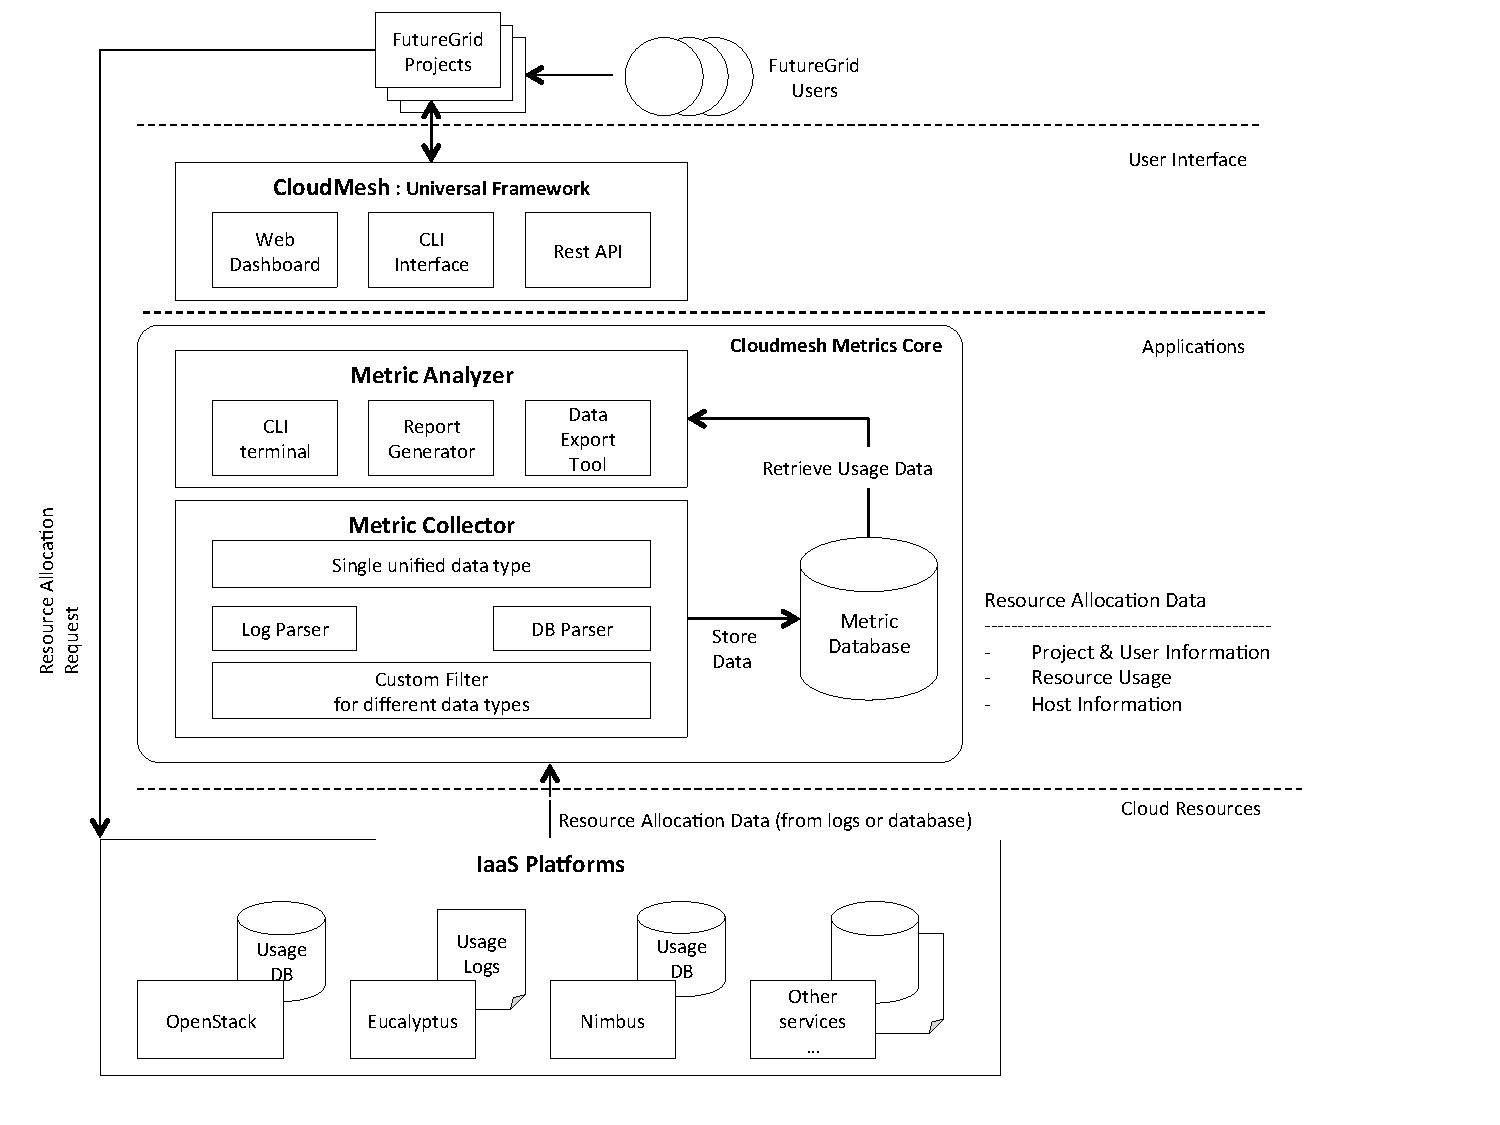
\includegraphics[width=1.0\columnwidth]{images/cloudmesh-metrics.pdf}
%  \caption{Design of Cloudmesh Metrics Architecture}
%  \label{F:metric-arch}
%\end{figure}

One of the base services needed is a data collector. It collects relevant data from a variety of sources including resource databases, logfiles, and data reporters. Hence, to integrate new cloud services into the data collectors we have to define a data model, as well as data sources that populate the data model with data. Currently data collectors are available for OpenStack, Eucalyptus, and Nimbus but not limited to these platforms. Dependent on the IaaS framework they obtain the data from different sources such as log files or data bases as listed in Table \ref{T:compare-iaas}. Information that is useful to be collected include detailed information about the virtual machines, the users and/or projects starting them, memory usage over the lifetime of the VM, errors associated with vms during runtime, or as startup. One of the issues to be addressed is if such data should be directly accessed in the production environment offered by the IaaS framework. Practical experience with FutureGrid has shown that the analysis of the data poses a significant amount of stress on the originating resource making it impractical to offer a detailed report and metric system on the original data sources. Hence it is important that we replicate it when the information we request is involved in a detailed analysis. For some smaler scale queries as the one posed by users direct access is sufficient and desirable in case of a live view of the system in order to provide information about how many VMs are currently running, on which system and by whom.



%\newcommand{\YES}{\checkmark}
%\newcommand{\NO}{\textopenbullet}
\newcommand{\YES}{\ding{51}}
\newcommand{\NO}{\ding{55}}
%\newcommand{\YES}{$\oplus$}
%\newcommand{\NO}{$\ominus$}


\begin{table}[h!]
  \caption{Measurement of IaaS on FutureGrid}\label{T:compare-iaas}
  ~\\
  \begin{small}
  \begin{tabularx}{\columnwidth}{|l|X|X|X|}
  \hline
                 & {\bf Nimbus} & {\bf OpenStack} & {\bf Eucalyptus} \\
    \hline
    \hline
    \multicolumn{4}{|l|}{\bf Documentation of the Data Sources} \\
    \hline
       & \NO & \YES & \YES \\
    \hline
    \hline
    \multicolumn{4}{|l|}{\bf Data Sources} \\
    \hline
         & sqlite3 & MySQL & Log Files \\
    \hline
    \hline
    \multicolumn{4}{|l|}{\bf Metrics} \\
    \hline
    ~~vCPU core & \YES & \YES & \YES \\
    ~~memory & \YES & \YES & \YES \\
    ~~disk & \YES & \YES & \YES \\
    ~~instance type   & \NO & \YES & \YES \\
    ~~host & \YES & \YES & \YES \\
    \hline
    \hline
    \multicolumn{4}{|l|}{\bf Account Management Features} \\
    \hline
    ~~Users     & \YES & \YES & \YES \\
    ~~Projects & \NO & \YES & \YES \\
    \hline
    \hline
    \multicolumn{4}{|l|}{\bf Cluster} \\
    \hline
    ~~Alamo  & \YES & \YES & \NO \\
    ~~Foxtrot & \YES & \NO & \NO \\
    ~~Hotel    & \YES & \YES & \NO \\
    ~~India     & \NO  & \YES & \YES \\
    ~~Sierra    & \NO & \YES & \YES \\
%    ~~Lima     & ?       &  ?      &  ?       \\   
    \hline
%    Region& \shortstack[l]{TACC$^1$, \\UF$^2$, \\UChicago$^3$, \\SDSC$^4$} & \shortstack[l]{TACC, \\IU$^5$, \\SDSC } & \shortstack[l]{IU, \\SDSC$^6$} \\
%    \hline
  \end{tabularx}\\
%  $^1$ Texas Advanced Computing Center \\
%  $^2$ University of Florida \\
%  $^3$ University of Chicago \\
%  $^4$ San Diego Supercomputing Center\\
%  $^5$ Indiana University\\
%  $^6$ in early 2014\\
\end{small}
\end{table}


\paragraph{Metric Analyzer}


\todo{READ}

The data collected provides the opportunity to analyze it for specific needs in a repeated fashion or provide filters and services for further specialized analysis. The FutureGrid metric framework provides therefore a metric analyzer component with a convenient interface for analyzing the data not only on an automated fashion, but also interactively through a simple metrics analyzer shell. Information of interest include yearly, monthly, weekly, usage information by user, project, resource, provider, and the agglomerated information. Our scripting environment provides this information and is run at predefined intervals or upon request. In future we will be enhancing the service to allow users to schedule queries to conduct specific analysis. To avoid repeated analysis, metric result caching is conducted. Thus if a query has been executed in the past the result is cached and returned without reanalysis (if not forced). To more easily facilitate fast and distributed calculation of the results by multiple users, we will base future versions of the Cloudmetric system on NoSQL database technologies.

\paragraph{Metric Interface}


\todo{READ}

Early on we recognized the access the information and the metrics must be provided through a variety of interfaces. This includes command shells, programming API's, REST interfaces, graphical user interfaces, and printable reports.

\begin{description}[leftmargin=*,itemsep=0pt,topsep=0pt]

\item[Interactive Command Shell.] To simplify the interactive use, we have developed a python command shell called CMD3 that allows the dynamic load of additional commands, thus making it ideal to define new analytic methods on the fly if they are not provided by the original toolkit.

\item[REST API.] To allow easy access from Web frameworks, but also integration form arbitrary programming languages, we are currently building access through a convenient REST API.

\item[Programming API.] We have provided a robust API interface in python to access the basic analytical functions useful for many users and reused by the interactive command shell and the REST service.

\item[Graphical Representation and Printable Reports.] ~\\ Using our basic API and command shell, we have integrated them into the Python sphinx framework \cite{brandl2009sphinx} to expose the metric data in a convenient form and present the data online via charts ~\cite{highsoft2012highcharts} or in a PDF report. As sphinx offers the export of data reports in PDF we leverage this framework and do not have to develop a separate frame work for it. The sphinx framework service is currently enhanced to allow customizable interactive queries to the metric and data sources. The data can be represented easily in various chart forms such as bar graphs, line charts, or pie charts. A template for generating a quarterly and yearly report of the data exists making adaptation to additional resources or other provider consortia easy. Furthermore, the data can be exported in a variety of formats such as JSON or csv making it possible to use other tools such as excel for data post processing.  In Table~\ref{T:iaas-with-graph} we are including a limited number of examples to demonstrate the various data representations of the Cloudmetric system that are exposed to the users.

\end{description}

\begin{table}[h!]
  \caption{Metric visualization with graphs}\label{T:iaas-with-graph}
  ~\\
  \begin{center}
  \begin{small}
  \begin{tabular}{|p{0.2\columnwidth}|p{0.7\columnwidth}|}
  \hline
  {\bf Example} & {\bf Description} \\
    \hline
    \adjustbox{valign=t}{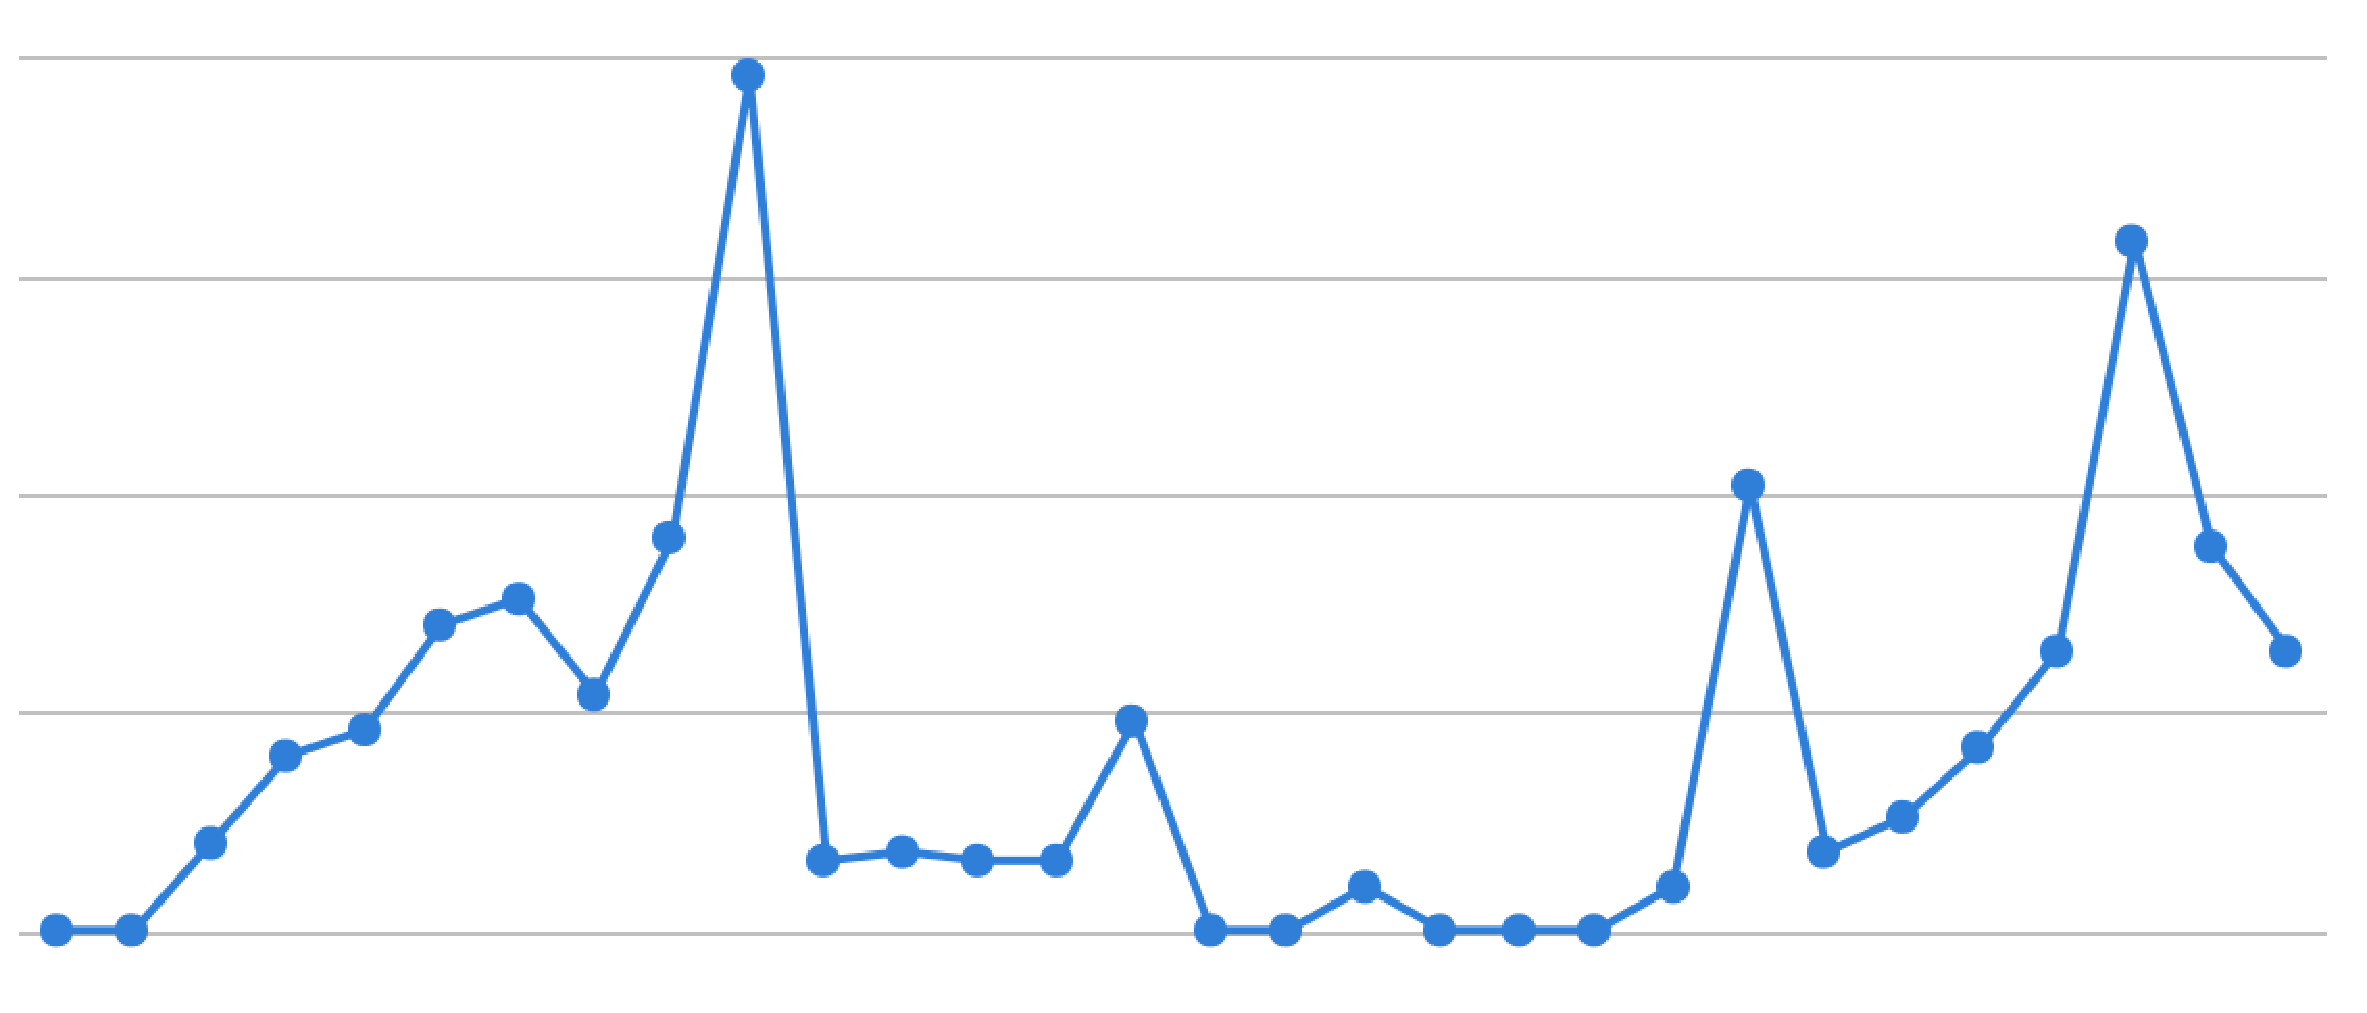
\includegraphics[width=0.2\columnwidth]{images/metric-line-chart.pdf}}
    &  
    Detailed display of virtual machine information including number
    of virtual machines, user count, memory utilization, disk
    utilization, project lead, etc. \\
    \hline
    \adjustbox{valign=t}{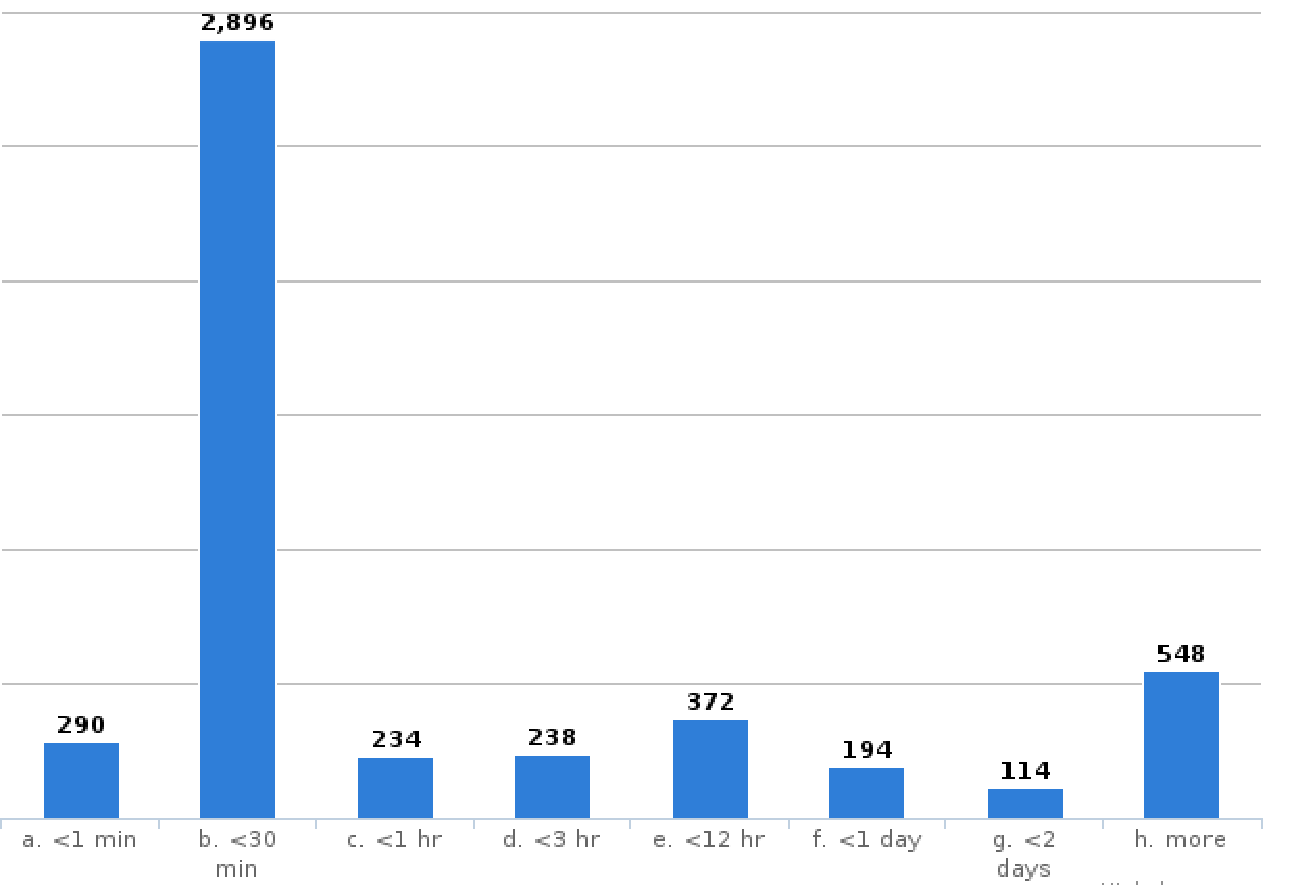
\includegraphics[width=0.2\columnwidth]{images/metric-histogram-chart.pdf}}
    & Summary information for periods to display aggregates of the
    metrics gathered by the system, such as number of vms by month for
    a user, project, or resource.  \\
    \hline
    \adjustbox{valign=t}{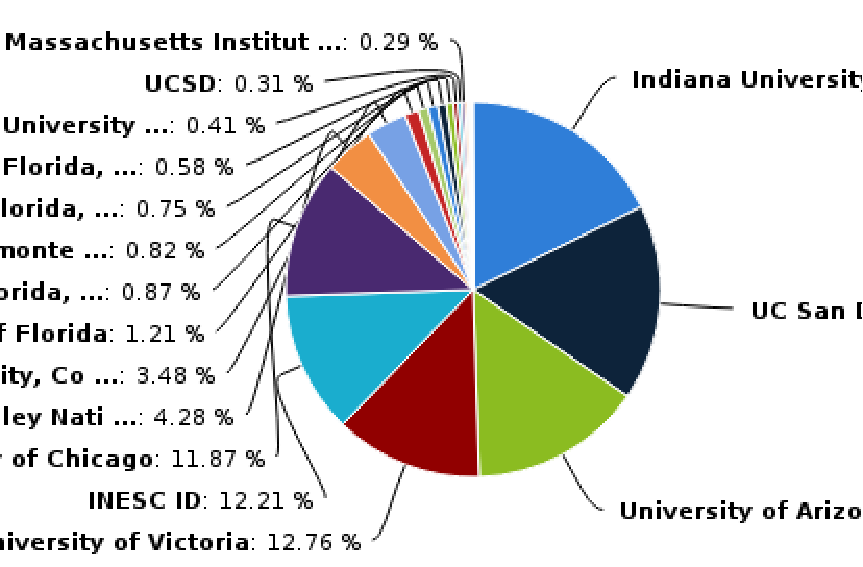
\includegraphics[width=0.2\columnwidth]{images/metric-pie-chart.pdf}}
    & Alternate representation of aggregated information in pie
    charts. \\
    \hline
    \adjustbox{valign=t}{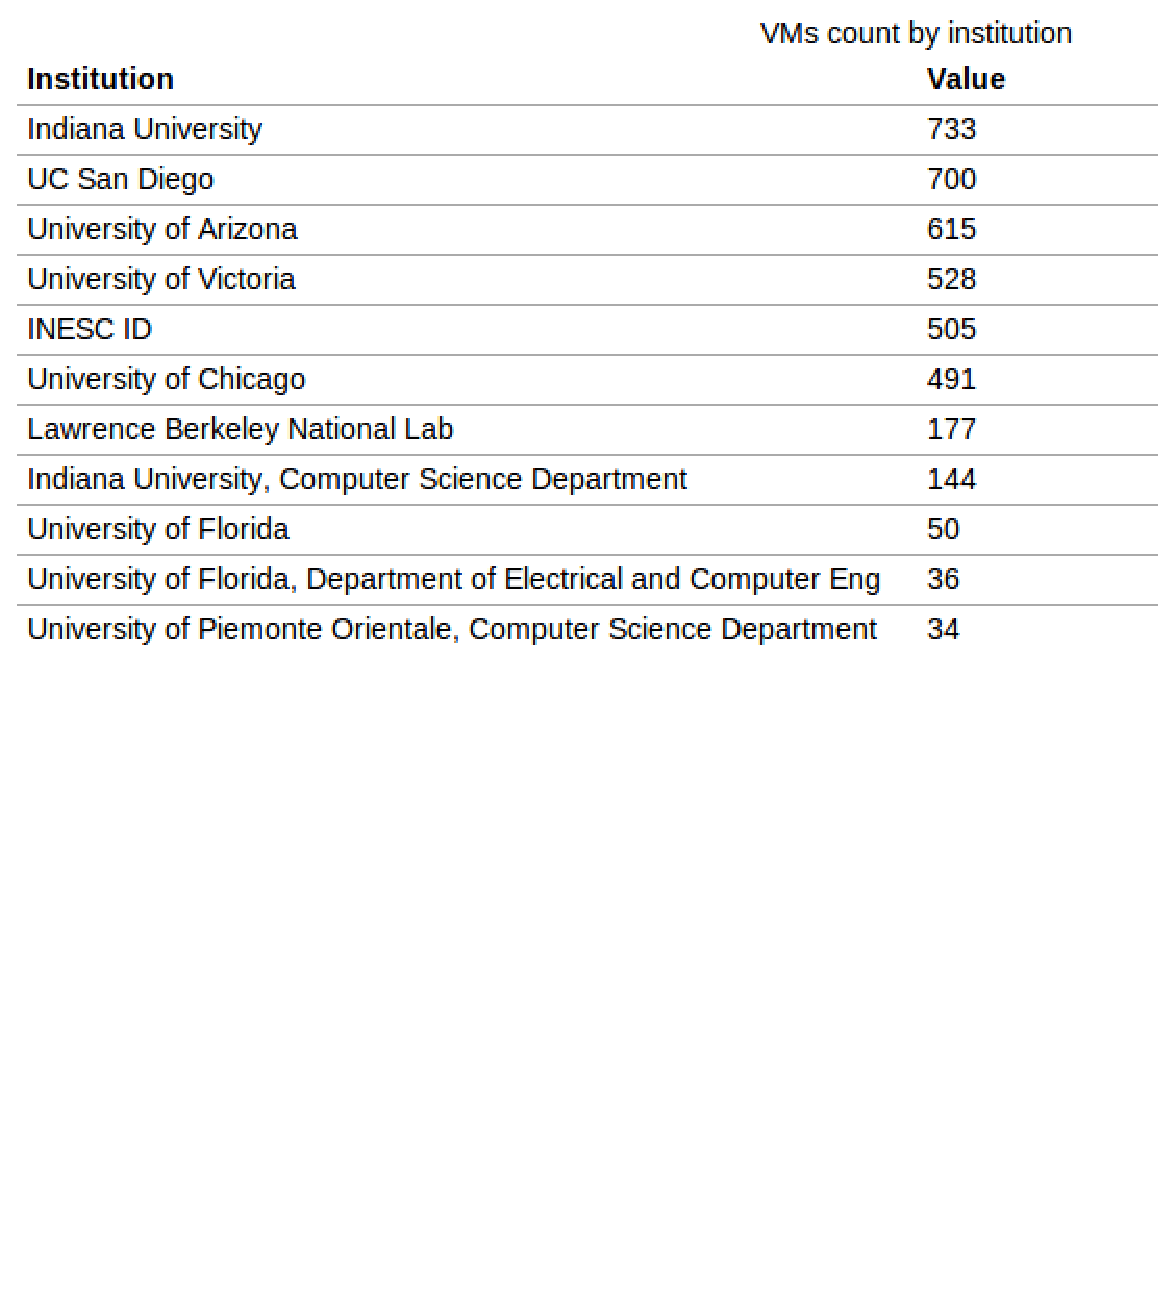
\includegraphics[width=0.2\columnwidth]{images/metric-table-chart.pdf}}
    & 
    Alternate representation of agglomerated information in a table
    (exporatble as csv or json). \\
    \hline
  \end{tabular}\\
\end{small}
\end{center}
\end{table}

\paragraph{Integration into XSEDE}

TBD

%%%%%%%%%%%%%%%%%%%%%%%%%%%%%%%%%%%%%%%%%%%%%%%%%%%%%%%%%%%%%%%%%%%%%%
\section{Conclusion}\label{S:conclusion}
%%%%%%%%%%%%%%%%%%%%%%%%%%%%%%%%%%%%%%%%%%%%%%%%%%%%%%%%%%%%%%%%%%%%%%

TBD
 
%%%%%%%%%%%%%%%%%%%%%%%%%%%%%%%%%%%%%%%%%%%%%%%%%%%%%%%%%%%%%%%%%%%%%% 
% Acknowledgment 
%%%%%%%%%%%%%%%%%%%%%%%%%%%%%%%%%%%%%%%%%%%%%%%%%%%%%%%%%%%%%%%%%%%%%% 


\section{Acknowledgments}

\todo{READ}

This material is based upon work supported in part by the National Science Foundation under Grant No. 0910812 and OCI 1025159.

\bibliographystyle{abbrvurl}
\bibliography{% 
bib/vonLaszewski-jabref.bib,%
bib/cyberaide-cloud,%
bib/cyberaide-metric} 

%\balancecolumns 
\end{document}
